
\begin{block}{Named Entity Recognition (CoNLL 2003)}
\begin{table}[t]
  {\small
%% NER 
\begin{tabular}{l r r r r r r }
%  \multicolumn{7}{c}{Named Entity Recognition}  \\
      \textbf{System} & \textbf{Latency/tok} & \textbf{Qs/tok} & \textbf{PER F$_1$} & \textbf{LOC F$_1$} & \textbf{ORG F$_1$} & \textbf{F$_1$}
    \\ \hline
    1-vote & 467 ms & 1.0 & 90.2 & 78.8 & 71.5 & 80.2
      \\ %\hline
    3-vote & 750 ms & 3.0 & 93.6 & 85.1 & 74.5 & 85.4
        \\ %\hline
    5-vote & 1350 ms & 5.0 & \textbf{95.5} & 87.7 & 78.7 & 87.3 
        \\ \hline
    Online & n/a & n/a & 56.9 & 74.6 & 51.4 & 60.9
        \\    %\hline
    Threshold & 414 ms & 0.61 & 95.2 & \textbf{89.8} & 79.8 & 88.3
        \\ %\hline
    \textbf{LENSE} & \textbf{267 ms} & \textbf{0.45} & 95.2 & 89.7 & \textbf{81.7} & \textbf{88.8} 
\end{tabular}
}
%\caption{Results on NER (CoNLL 2003) comparing latencies, queries per token (Qs/tok) and per-class \fone{} scores.}
\label{tbl:results}
\end{table}

  \begin{center}
    \colorbox{white}{
    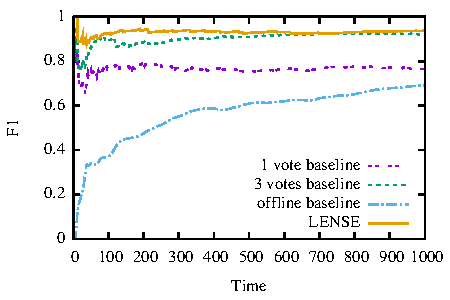
\includegraphics[width=0.45\columnwidth]{ner_2_class/f1_plot/f1_vs_time.pdf}
    }
    \colorbox{white}{
    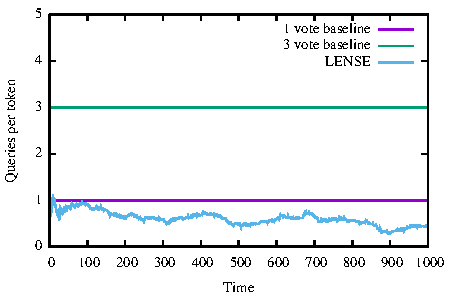
\includegraphics[width=0.45\columnwidth]{ner_2_class/cost_plot/cost_vs_time.pdf}
    }
  \end{center}

  \begin{exampleblock}{Takeaway}
      On-the-job learning is capable of making consistently accurate predictions while reducing annotation costs.
  \end{exampleblock}
\end{block}
\vfill

\begin{block}{Sentiment}
    \begin{minipage}[t]{.43\columnwidth}
      \colorbox{white}{
      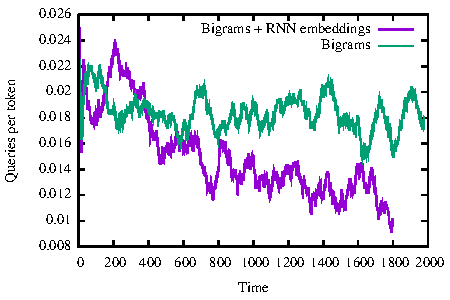
\includegraphics[width=\textwidth]{sentiment_cost_per_token_vs_time/cost_per_token_vs_time.pdf}
      }
    \end{minipage}
    \quad
    \begin{minipage}[t]{.45\columnwidth}
      \begin{tabular}[b]{l  r  r  r  r}
          %\hline
          \textbf{System} & \textbf{Latency} & \textbf{Qs/ex} & \textbf{Acc.} \\ \hline
          5-vote & 13.5 s & 5.00 & 98.7 \\ %\hline
          \multicolumn{5}{c}{\textsc{unigrams}} \\ \hline
          Online & n/a & n/a & 78.1 \\ %\hline
          Threshold & 10.9 s & 2.99 & 95.9 \\ %\hline
          \textbf{LENSE} & 11.7 s & 3.48 & 98.6 \\ %\hline
          \multicolumn{5}{c}{\textsc{rnn}} \\ \hline
          Online & n/a & n/a & 85.0 \\ %\hline
          Threshold & 11.0 s & 2.85 & 96.0 \\ %\hline
          \textbf{LENSE} & 11.0 s & 3.19 & 98.6 \\% \hline
      \end{tabular}
    \end{minipage}%

  \begin{exampleblock}{Takeaway}
      On-the-job learning will maintain accuracy even if the model lacks the capacity to.
  \end{exampleblock}
\end{block}
\vfill

\begin{block}{Conclusions and Future Work}
  \begin{itemize}
    \item Consider on-the-job learning to get accurate labels on your
      next project for cheap. 
    \item Easy to use open-source implementation, LENSE, available!
    \item Future directions include improving confidence estimation, 
      learning from measurements and more applications.
  \end{itemize}
\end{block}
\vfill

